% ============================================================
%  Mohammad Vazir Panah -- Academic / Research CV (fixed)
% ============================================================

\documentclass[10pt, a4paper]{article}

% -- Encoding & font -------------------------------------------------
\usepackage[T1]{fontenc}
\usepackage[utf8]{inputenc}
\usepackage{microtype}
\usepackage{helvet}
\renewcommand{\familydefault}{\sfdefault}

% -- Page geometry ---------------------------------------------------
\usepackage[
  top    = 1.75cm,
  bottom = 1.4cm,
  left   = 1.8cm,
  right  = 1.8cm
]{geometry}

% -- Colours ---------------------------------------------------------
\usepackage[table]{xcolor}
\definecolor{navy}{HTML}{1C3557}
\definecolor{accent}{HTML}{2563A8}
\definecolor{midtext}{HTML}{4A5568}
\definecolor{lightbg}{HTML}{EEF2F7}
\definecolor{hdrbg}{HTML}{DDE8F5}
\definecolor{rulecol}{HTML}{CBD5E0}

% -- Hyperlinks ------------------------------------------------------
\usepackage[
  colorlinks = true,
  urlcolor   = accent,
  linkcolor  = accent,
  pdftitle   = {Mohammad VazirPanah -- CV},
  pdfauthor  = {Mohammad VazirPanah}
]{hyperref}
\urlstyle{same}

% -- Graphics & TikZ -------------------------------------------------
\usepackage{graphicx}
\usepackage{tikz}
\usetikzlibrary{calc}

% -- Tables ----------------------------------------------------------
\usepackage{tabularx}
\usepackage{array}

% -- Lists -----------------------------------------------------------
\usepackage{enumitem}
\setlist[itemize]{
  leftmargin = 1.3em,
  itemsep    = 0.5pt,
  topsep     = 1.8pt,
  parsep     = 0pt,
  label      = \textbullet
}

% -- Paragraph spacing -----------------------------------------------
\setlength{\parindent}{0pt}
\setlength{\parskip}{0pt}
\emergencystretch=1em

% -- Section headers -------------------------------------------------
\usepackage{titlesec}
\titleformat{\section}[block]
  {\normalfont\bfseries\fontsize{10}{13}\selectfont\color{navy}}
  {}
  {0pt}
  {\tikz[baseline=-1pt,inner sep=0pt]{\fill[accent](0,0)rectangle(3pt,10pt);}\hspace{6pt}}
  [\vspace{-9pt}{\color{rulecol}\rule{\linewidth}{0.5pt}}]
\titlespacing*{\section}{0pt}{10pt}{5pt}
\newcommand{\firstsection}[1]{\section{#1}}

% -- Footer ----------------------------------------------------------
\usepackage{fancyhdr}
\pagestyle{fancy}
\fancyhf{}
\renewcommand{\headrulewidth}{0pt}
\fancyfoot[C]{%
  \begin{tikzpicture}[remember picture,overlay]
    \fill[navy](current page.south west)
      rectangle($(current page.south east)+(0,3pt)$);
  \end{tikzpicture}%
  \textcolor{midtext}{\scriptsize Page \thepage}%
}
\setlength{\footskip}{20pt}

% -- Full-bleed header ----------------------------------------------
\usepackage{eso-pic}

\newlength{\hdrH}   \setlength{\hdrH}{4.1cm}
\newlength{\padX}   \setlength{\padX}{1.8cm}
\newlength{\photoD} \setlength{\photoD}{2.75cm}

\AddToShipoutPictureFG*{%
  \begin{tikzpicture}[remember picture, overlay]
    \fill[hdrbg]
      (current page.north west)
      rectangle
      ($(current page.north east)+(0,-\hdrH)$);

    \fill[navy]
      (current page.north west)
      rectangle
      ($(current page.north east)+(0,-4pt)$);

    \draw[navy, line width=1.8pt]
      ($(current page.north west)+(0,-\hdrH)$) --
      ($(current page.north east)+(0,-\hdrH)$);

    \begin{scope}
      \clip ($(current page.north east)+(-\padX-\photoD/2,-\hdrH/2)$)
            circle(\photoD/2);
      \node at ($(current page.north east)+(-\padX-\photoD/2,-\hdrH/2)$)
            {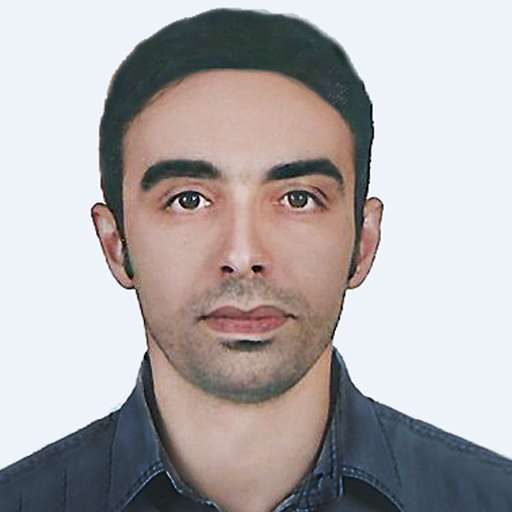
\includegraphics[width=\photoD]{profile.png}};
    \end{scope}
    \draw[white, line width=1.8pt]
      ($(current page.north east)+(-\padX-\photoD/2,-\hdrH/2)$)
      circle(\photoD/2);

    \node[
      anchor    = north west,
      inner sep = 10pt,
      text width= \dimexpr\paperwidth - 2\padX - \photoD - 0.7cm\relax
    ] at ($(current page.north west)+(\padX, -4pt-0.18cm)$) {%
      {\fontsize{22}{26}\selectfont\bfseries\color{navy}
        Mohammad VazirPanah}\\[5pt]
      % {\fontsize{9.2}{13}\selectfont\itshape\color{accent}
      %   Embedded Systems \& High-Performance Computing \textperiodcentered\
      %   University of Salerno}\\[5pt]
      {\color{rulecol}\rule{\linewidth}{0.4pt}}\\[5pt]
      {\fontsize{8.8}{13}\selectfont\color{midtext}
        Via Giuseppe De Falco 25, 84084 Fisciano (SA), Italy
        \,\textperiodcentered\,
        \href{tel:+393896646511}{(+39) 389\,664\,6511}}\\[4pt]
      {\fontsize{8.8}{13}\selectfont\color{accent}
        \href{mailto:mohammad.vazirpanah@gmail.com}{mohammad.vazirpanah@gmail.com}
        \,\textperiodcentered\,
        \href{https://www.linkedin.com/in/mohammadvazirpanah}{LinkedIn}
        \,\textperiodcentered\,
        \href{https://mohammadvazirpanah.github.io/}{Website}}\\[4pt]
      {\fontsize{8.8}{13}\selectfont\color{midtext}
        Nationality: Iranian
        \,\textperiodcentered\,
        DOB: 23 Apr 1994}%
    };
  \end{tikzpicture}%
}

% -- Helpers ---------------------------------------------------------
\newcommand{\IfNonEmptyTF}[3]{%
  \if\relax\detokenize{#1}\relax
    #3%
  \else
    #2%
  \fi
}

\newcommand{\cventry}[4]{%
  \IfNonEmptyTF{#1}{%
    \begin{tabularx}{\linewidth}{@{}>{\raggedright\arraybackslash}X >{\raggedleft\arraybackslash}p{3.15cm}@{}}
      \textbf{#2} & {\itshape\small\textcolor{accent}{#1}} \\
    \end{tabularx}\par%
  }{%
    \textbf{#2}\par
  }%
  \IfNonEmptyTF{#3}{%
    \vspace{1pt}{\itshape\textcolor{midtext}{#3}}\par
  }{}%
  \IfNonEmptyTF{#4}{%
    \vspace{2pt}%
    \begin{itemize}
      #4
    \end{itemize}
  }{}%
  \vspace{5pt}%
}

\newcommand{\pubentry}[4]{%
  \vspace{2pt}\noindent
  \begin{tabularx}{\linewidth}{@{}p{1.0cm}>{\raggedright\arraybackslash}X@{}}
    \raisebox{0pt}[0pt][0pt]{%
      \begin{tikzpicture}[baseline=2pt, inner sep=0pt]
        \node[fill=navy, rounded corners=2pt,
              inner xsep=5pt, inner ysep=2.5pt,
              text=white,
              font=\bfseries\fontsize{7.5}{9}\selectfont] {#1};
      \end{tikzpicture}%
    } &
    {\textbf{#3}\par
    \vspace{1pt}{\small\itshape\textcolor{midtext}{#2}}\par
    \vspace{1pt}{\fontsize{8.2}{11}\selectfont\textcolor{midtext}{#4}}} \\
  \end{tabularx}
  \vspace{4pt}%
}

\newenvironment{shadedtable}[1]{%
  \vspace{2pt}%
  \rowcolors{1}{white}{lightbg}%
  \tabularx{\linewidth}{#1}%
}{%
  \endtabularx
  \rowcolors{1}{}{}%
  \vspace{4pt}%
}

% ============================================================
\begin{document}
\vspace*{2.2cm}
% ============================================================

\firstsection{Research Interests}

Embedded Systems, Robotics, HPC, RISC-V Architectures, Real-Time Heterogeneous Platforms
% Embedded Systems, High-Performance Computing, and RISC-V Architectures for Real-Time Heterogeneous Systems
\section{Education}

\cventry{Sep 2019 -- Oct 2022}
  {M.Sc. in Computer Engineering --- Computer Systems Architecture}
  {Shahid Beheshti University, Tehran, Iran}
  {
    \item GPA: 3.79\,/\,4.00
    \item Thesis: \textit{A Framework for Modeling Self-Aware Cyber-Physical Systems with SystemC}
    \item Supervisor: Dr. Seyed-Hosein Attarzadeh-Niaki
  }

\cventry{Sep 2012 -- May 2016}
  {B.Sc. in Computer Engineering --- Hardware Engineering}
  {Birjand University, Birjand, Iran}
  {
    \item GPA: 3.40\,/\,4.00
    \item Project: \textit{Simulation and Programming the Alpha Rex Human-Robot Produced by Lego Company}
  }

\section{Work Experience}

\cventry{2023 -- 2026}
  {Research Fellow}
  {University of Salerno --- Dept. of Computer Science, ISISLab, Salerno, Italy}
  {
    \item Scientific Responsible: Prof. Biagio Cosenza
    \item Focus on High-Performance Computing and RISC-V architectures
    \item Contributed to \href{https://librert.di.unisa.it/}{LibreRT}: developing and deploying real-time applications on embedded CPUs and GPUs
    \item Evaluated compiler performance (GCC, LLVM) on RISC-V vector boards
    \item Deployed SoC boards; managed experiments with Git, Docker, CI; documented setups for reproducibility
  }

\cventry{2013 -- 2015}
  {Instructor}
  {Sepehr Educational Institutions, Kashmar, Iran}
  {
    \item Delivered theoretical and practical instruction in C++ programming
    \item Taught ICDL (International Computer Driving License) skills
    \item Taught CorelDRAW and Adobe FreeHand, focusing on vector graphics
  }

\cventry{2014 -- 2015}
  {Education Intern}
  {Abooreyhan Company, Kashmar, Iran}
  {
    \item Hardware/software troubleshooting, diagnostics, and component replacement
    \item Assembled and configured PCs; software installation and system setup
  }

\section{Academic Experience}

\textbf{Teaching Assistantships}\\[5pt]
\begin{tabularx}{\linewidth}{@{}>{\itshape\raggedright\arraybackslash}X >{\raggedright\arraybackslash}p{2.2cm} >{\raggedleft\arraybackslash}p{2.1cm}@{}}
  Design \& Analysis of Real-Time Embedded Systems & SBU & 2021 \\
  System-on-Chip & SBU & 2020, 2021 \\
  Advanced Computer Architecture & SBU & 2021 \\
  Fundamentals of Embedded \& Real-Time Systems & SBU & 2020 \\
  Computer Architecture & Birjand Univ. & 2016 \\
\end{tabularx}
\rowcolors{1}{}{}

\vspace{8pt}
\textbf{Laboratory Memberships}
\begin{itemize}
  \item ISISLab --- HPC Group, University of Salerno, Italy
  \item SBU Cyber-Physical Systems Lab Research Team, Tehran, Iran
\end{itemize}

\vspace*{1cm}

% \section{Publications}

% \pubentry{2026}
%   {B. Cosenza, F. Terraneo, G. Agosta, L. Carpentieri, D. Cattaneo, \textbf{M. VazirPanah}, N. Nicolosi}
%   {LibreRT: Portable Heterogeneous Real-Time Programming for the Embedded Computing Continuum}
%   {23rd ACM International Conference on Computing Frontiers (CF), Special Sessions \textperiodcentered\ 2026}

% \pubentry{2025}
%   {L. Carpentieri, \textbf{M. VazirPanah}, B. Cosenza}
%   {A Performance Analysis of Autovectorization on RVV RISC-V Boards}
%   {PDP --- 33rd Euromicro International Conference on Parallel, Distributed, and Network-Based Processing, IEEE \textperiodcentered\ 2025}
%   % {DOI: 10.1109/PDP66500.2025.00026}

% \pubentry{2023}
%   {S.-H. Attarzadeh-Niaki, \textbf{M. Vazirpanah}}
%   {System-Level Modeling of Dynamic Applications with Scenario-Aware Dataflow Graphs}
%   {Journal of Innovations in Computer Science and Engineering (JICSE), Shahid Beheshti University \textperiodcentered\ 2023}

% \pubentry{2022}
%   {\textbf{M. Vazirpanah}, S.-H. Attarzadeh-Niaki, A. Salimi-Badr}
%   {ROS-Based Co-Simulation for Formal Cyber-Physical Robotic System Design}
%   {27th International Computer Conference, Computer Society of Iran (CSICC), IEEE \textperiodcentered\ 2022}
%   %DOI: 10.1109/CSICC55295.2022.9780500


\section{Publications}

\pubentry{2026}
  {B. Cosenza, F. Terraneo, G. Agosta, L. Carpentieri, D. Cattaneo, \textbf{M. VazirPanah}, N. Nicolosi}
  {\href{https://doi.org/10.1145/3801488.3806240}{LibreRT: Portable Heterogeneous Real-Time Programming for the Embedded Computing Continuum}}
  {23rd ACM International Conference on Computing Frontiers (CF), Special Sessions \textperiodcentered\ 2026}

\pubentry{2025}
  {L. Carpentieri, \textbf{M. VazirPanah}, B. Cosenza}
  {\href{https://doi.org/10.1109/PDP66500.2025.00026}{A Performance Analysis of Autovectorization on RVV RISC-V Boards}}
  {PDP --- 33rd Euromicro International Conference on Parallel, Distributed, and Network-Based Processing, IEEE \textperiodcentered\ 2025}

\pubentry{2023}
  {S.-H. Attarzadeh-Niaki, \textbf{M. VazirPanah}}
  {\href{https://jicse.sbu.ac.ir/article_104210_2b02304940f4fcd17c19d38cfc08e528.pdf}{System-Level Modeling of Dynamic Applications with Scenario-Aware Dataflow Graphs}}
  {Journal of Innovations in Computer Science and Engineering (JICSE), Shahid Beheshti University \textperiodcentered\ 2023}

\pubentry{2022}
  {\textbf{M. VazirPanah}, S.-H. Attarzadeh-Niaki, A. Salimi-Badr}
  {\href{https://doi.org/10.1109/CSICC55295.2022.9780500}{ROS-Based Co-Simulation for Formal Cyber-Physical Robotic System Design}}
  {27th International Computer Conference, Computer Society of Iran (CSICC), IEEE \textperiodcentered\ 2022}

\section{Selected Projects}

\cventry{2023 -- 2026}
    {LibreRT --- Portable Heterogeneous Real-Time Programming for the Embedded Computing Continuum}
    {\href{https://librert.di.unisa.it/}{Researcher, Italian PRIN 2022-funded project}}
    {
      \item Developed and evaluated real-time applications for heterogeneous embedded CPU/GPU platforms
      \item Implemented solutions using SYCL, OpenMP, OpenCL, and RISC-V boards
    }

\cventry{2025}
  {RISC-V Benchmark Suite}
  {\href{https://github.com/unisa-hpc/RISCV-bench}{Open-source project GitHub}}
  {
    \item Designed and implemented benchmarks for RISC-V and RVV architectures
    \item Evaluated performance across multiple GCC and LLVM compiler versions
  }

\cventry{2022}
  {Self-Aware CPS Modeling Framework}
  {M.Sc. Thesis — \href{https://github.com/mohammadvazirpanah/ForSyDe-SystemC/tree/sadf-dstarlite-ros}{Open-source project GitHub} — based on \href{https://github.com/forsyde/ForSyDe-SystemC}{ForSyDe-SystemC Modeling Framework}}
  {
    \item Designed and implemented a self-aware cyber-physical system model using ForSyDe-SystemC and ROS-Gazebo co-simulation
    \item Developed an SADF-based model and contributed extensions to the ForSyDe-SystemC library
  }

\cventry{2020}
  {Railroad System Verification with NuSMV}
  {Course Project, M.Sc. Design and Analysis of Real-Time Embedded Systems}
  {
    \item Modeled and verified a railroad control system using NuSMV
    \item Checked safety and liveness properties through formal verification
  }

  
\cventry{2019}
  {FIR Filter and Tiny YOLO v1 on FPGA}
  {Course Project, M.Sc. System-on-Chip, DE0-Nano / DE10 Intel FPGA Board}
  {
    \item Designed and implemented a FIR filter IP core in Quartus with an Avalon-MM interface
    \item Implemented real-time Tiny YOLO v1 object detection on FPGA under resource constraints
  }


  
\section{Technical Skills}

\begin{shadedtable}{@{}>{\bfseries\raggedright\arraybackslash}p{4.3cm} X@{}}
  Programming & C, C++, Python, MATLAB, Assembly \\
  Parallel Models & OpenMP, OpenCL, SYCL \\
  Hardware / Embedded & FPGA, RISC-V, VHDL, Verilog, SystemC, FreeRTOS \\
  Simulation \& EDA & Gem5, QEMU, OVPsim, Quartus, ModelSim, MATLAB-Simulink, Ansys SCADE \\
  Robotics & ROS, Gazebo \\
  DevOps \& Tools & Git, Docker, Linux, \LaTeX, OpenModelica, NuSMV, UPPAAL \\
\end{shadedtable}

\vspace{1cm}
\section{Honours and Awards}

\cventry{2020}
  {National R\&D Research Grant Winner}
  {R\&D Center, Mobile Telecommunication Company of Iran (MCI)}
  {
    \item Awarded among competing Master's and PhD students in a national grant competition
  }

\cventry{2016}
  {Top Computer Engineering Student}
  {Birjand University}
  {
    \item Ranked in the top 15\% of B.Sc. Computer Engineering graduates
  }

\section{Conference Participation}

\cventry{Mar 2025}
  {33rd Euromicro International Conference on Parallel, Distributed, and Network-Based Processing (PDP)}
  {Co-author and attendee --- Turin, Italy}
  {
    \item Co-author of the paper: \textit{A Performance Analysis of Autovectorization on RVV RISC-V Boards}
    % \item Paper presented at the conference by a co-author
  }

\cventry{Feb 2022}
  {27th International Computer Conference, Computer Society of Iran (CSICC)}
  {Presenter --- Sharif University of Technology, Tehran, Iran}
  {
    \item Presented the paper: \textit{ROS-Based Co-Simulation for Formal Cyber-Physical Robotic System Design}
  }


\section{Language Skills}

\begin{shadedtable}{@{}>{\bfseries}p{2.4cm} X@{}}
  Persian & Native \\
  English & Proficient --- (Listening, Reading, Writing, Speaking) \\
  Italian & Basic --- (Listening, Reading, Writing, Speaking) \\
\end{shadedtable}

\section{References}

\begin{tabularx}{\linewidth}{@{} X X X @{}}
  \textbf{Prof. Biagio Cosenza} &
  \textbf{Prof. Vittorio Scarano} &
  \textbf{Dr. S.-H. Attarzadeh-Niaki} \\[2pt]
  \textit{Research Supervisor} &
  \textit{Head of ISISLab} &
  \textit{M.Sc. Supervisor} \\[2pt]
  University of Salerno, Italy &
  University of Salerno, Italy &
  Shahid Beheshti University, Iran \\[2pt]
  \href{mailto:bcosenza@unisa.it}{bcosenza@unisa.it} &
  \href{mailto:vitsca@unisa.it}{vitsca@unisa.it} &
  \href{mailto:h_attarzadeh@sbu.ac.ir}{h\_attarzadeh@sbu.ac.ir} \\
\end{tabularx}

\end{document}